\section{PTracking Algorithm}

\begin{frame}
	\frametitle{Distributed Particle Filtering for Multi-Camera Object Tracking}
	
	\Large
	
	\begin{block}{Idea}
		Achieving both a \textbf{high} precision and a \textbf{high} robustness, as a
		global method does, while keeping a \textbf{low} computational load in order to
		obtain \textbf{real-time} performance, as recursive methods do
	\end{block}
\end{frame}

\begin{frame}
	\frametitle{PTracking algorithm}
	
	\only<1->
	{
		\Large
		Each agent runs a two-tiered distributed algorithm
	}
	
	\begin{columns}
		\column{0.4\textwidth}
		\centering
		
		\only<1->
		{
			\vspace{0.7cm}
		}
		
		\only<1->
		{
			\begin{tikzpicture}
				\node at (0,0) [draw=black,ultra thick,inner sep=0pt]  {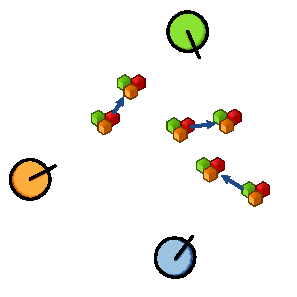
\includegraphics[scale=0.75]{Figures/Mamot}};
			\end{tikzpicture}
		}
		
		\column{0.2\textwidth}
		\centering
		
		\only<2->
		{
			\begin{tikzpicture}
				\node at (0,0) [draw=white,ultra thick,inner sep=0pt]  {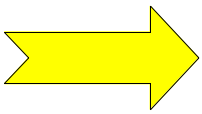
\includegraphics[scale=0.3]{Figures/ArrowRight.png}};
			\end{tikzpicture}
		}
		
		\column{0.4\textwidth}
		\centering
		
		\only<2>
		{
			\begin{tikzpicture}
				\node at (0,0) [draw=black,ultra thick,inner sep=0pt]  {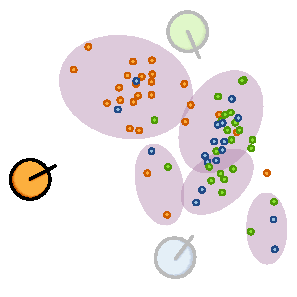
\includegraphics[scale=0.75]{Figures/Mamot2}};
			\end{tikzpicture}
		}
		
		\only<2>
		{
			\vspace{-0.7cm}
		}
		
		\only<3>
		{
			\begin{tikzpicture}
				\node at (0,0) [draw=black,ultra thick,inner sep=0pt]  {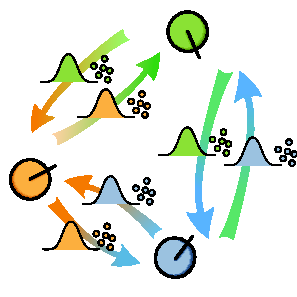
\includegraphics[scale=0.75]{Figures/Mamot3}};
			\end{tikzpicture}
		}
		
		\only<3>
		{
			\vspace{-0.7cm}
		}
		
		\only<4>
		{
			\begin{tikzpicture}
				\node at (0,0) [draw=black,ultra thick,inner sep=0pt]  {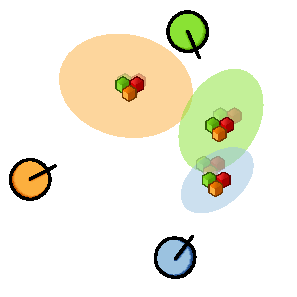
\includegraphics[scale=0.75]{Figures/Mamot4}};
			\end{tikzpicture}
		}
		
		\only<4>
		{
			\vspace{-0.7cm}
		}
	\end{columns}
\end{frame}

\begin{frame}
	\frametitle{Evaluating a Tracking Algorithm}
	
	\Large
	
	\vspace{0.3cm}
	
	The CLEAR MOT \cite{Kasturi09} metrics \emph{MOTA} and \emph{MOTP} are the de-facto
	standard for evaluating a tracking method:
	
	\vspace{0.2cm}
	
	\large
	
	\begin{equation*}
		MOTA = 1 - \frac{\sum_{t=1}^{N_{frames}} (c_m(m_t) + c_f(fp_t) + cs(ID\mbox{-}SWITCHES_t))}{\sum_{t=1}^{N_{frames}} N_G^{(t)}}
	\end{equation*}
	
	\vspace{0.4cm}
	
	\begin{equation*}
		MOTP = \frac{\sum_{i=1}^{N_{mapped}} \sum_{t=1}^{N_{frames}^{(t)}} \Big [ \frac{| G_i^{(t)} \cap D_i^{(t)} |}{| G_i^{(t)} \cup D_i^{(t)} |} \Big ] }{\sum_{t=1}^{N_{frames}} N_{mapped}^{(t)}}
	\end{equation*}
\end{frame}

\begin{frame}
	\frametitle{Application Field}
	
	\vspace{0.01cm}
	
	\begin{itemize}
		\item Single-Agent, Multi-Object
	\end{itemize}
	
	\vspace{-0.45cm}
	
	\begin{columns}[t]
		\only<1->
		{
			\column{0.75\textwidth}
			
			\begin{block}{Boat}
				automatic surveillance system for the maritime domain
			\end{block}
			
			\column{0.2\textwidth}
		}
	\end{columns}
	
	\centering
	\vspace{0.3cm}
	
	\begin{center}
		\begin{tikzpicture}
			\node at (0,0) [draw=black,ultra thick,inner sep=0pt]  {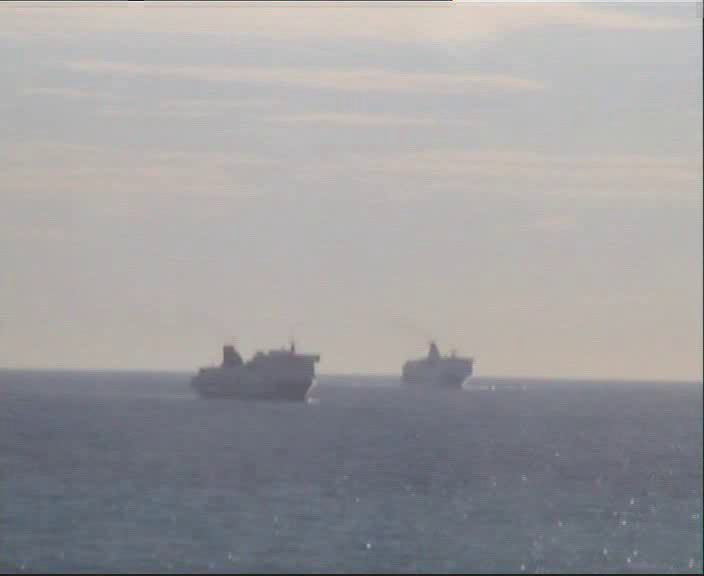
\includegraphics[height=3.1cm]{Figures/Boat-1}};
			\node at (4,0) [draw=black,ultra thick,inner sep=0pt]  {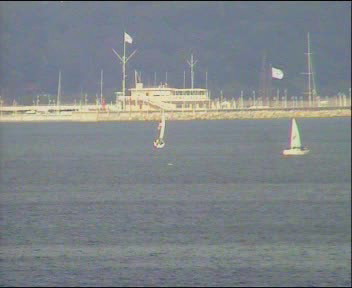
\includegraphics[height=3.1cm]{Figures/Boat-2}};
			\node at (8,0) [draw=black,ultra thick,inner sep=0pt]  {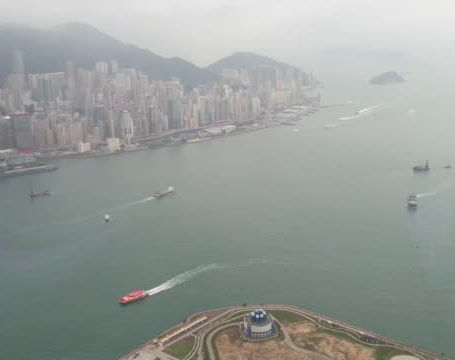
\includegraphics[height=3.1cm]{Figures/Boat-3}};
		\end{tikzpicture}
	\end{center}
\end{frame}

\begin{frame}
	\frametitle{Quantitative Evaluation on the Maritime Domain}
	
	\begin{table}[!t]
		\renewcommand{\arraystretch}{1.3}
		\caption{Tracking performance on the maritime domain. MOTA (larger the better)
				 considers the number of missed detections, the number of false positives
				 and the switches of identities. MOTP (larger the better) considers the
				 precision of the detections.}
		\centering
		\vspace{0.2cm}
		
		\begin{tabular}{ccc}
			\hline
			\hline
			\textbf{Video} & \textbf{MOTA} & \textbf{MOTP} \\
			\hline
			occlusions-1.avi & 0.815 & 0.613 \\
			\hline
			occlusions-2.avi & 0.910 & 0.554 \\
			\hline
			high-view.avi & 0.910 & 0.604 \\
			\hline
		\hline
		\end{tabular}
	\end{table}
\end{frame}

\begin{frame}
	\frametitle{Application Field}
	
	\vspace{0.24cm}
	
	\begin{itemize}
		\item Multi-Agent, Single-Object
	\end{itemize}
	
	\vspace{-0.45cm}
	
	\begin{columns}[t]
		\only<1->
		{
			\column{0.75\textwidth}
			
			\begin{block}{Soccer robots}
				used to solve the localization field symmetry problem
			\end{block}
			
			\column{0.2\textwidth}
		}
	\end{columns}
	
	\centering
	\vspace{0.3cm}
	
	\begin{tikzpicture}
				\node at (0,0) [draw=black,ultra thick,inner sep=0pt]  {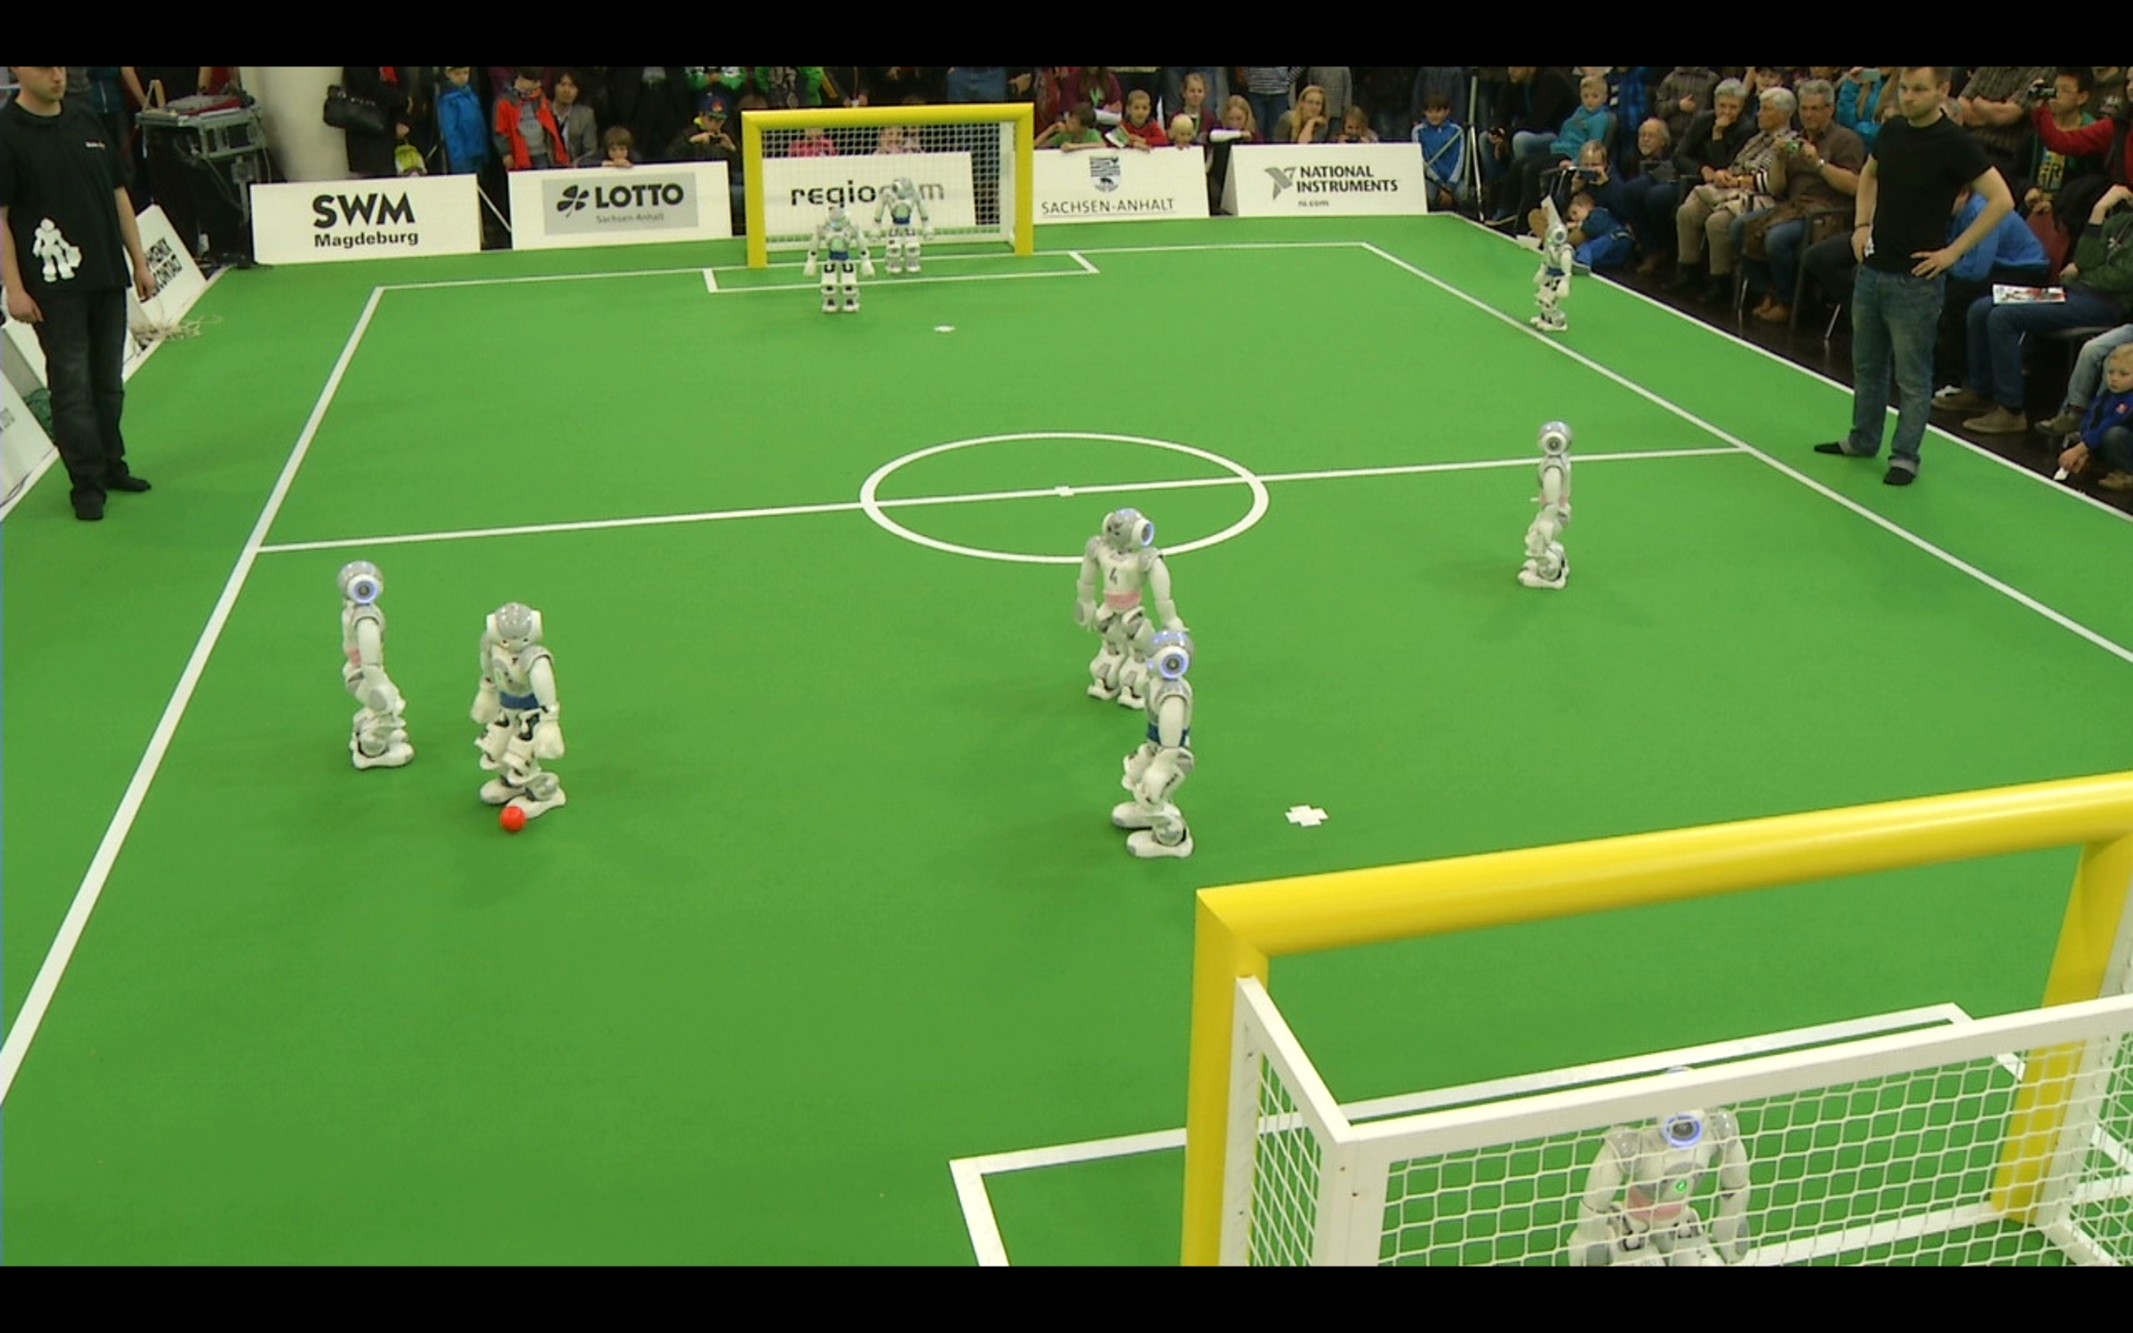
\includegraphics[scale=0.19]{Figures/Naos}};
	\end{tikzpicture}
	
\end{frame}

\begin{frame}
	\frametitle{Application Field}
	
	\vspace{-0.16cm}
	
	\begin{itemize}
		\item Multi-Agent, Multi-Object
	\end{itemize}
	
	\vspace{-0.45cm}
	
	\begin{columns}[t]
		\only<1->
		{
			\column{0.75\textwidth}
			
			\begin{block}{PETS 2009 data set}
				tracking of individuals within a crowd
			\end{block}
			
			\column{0.2\textwidth}
		}
	\end{columns}
	
	\centering
	\vspace{0.3cm}
	
	\begin{center}
		\begin{tikzpicture}
			\node at (0,0) [draw=black,ultra thick,inner sep=0pt]  {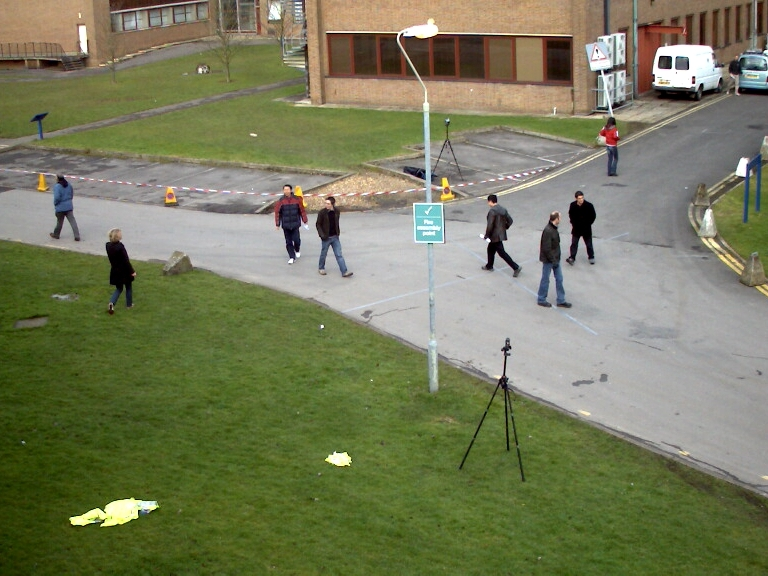
\includegraphics[height=2.85cm]{Figures/PETS2009-1}};
			\node at (4,0) [draw=black,ultra thick,inner sep=0pt]  {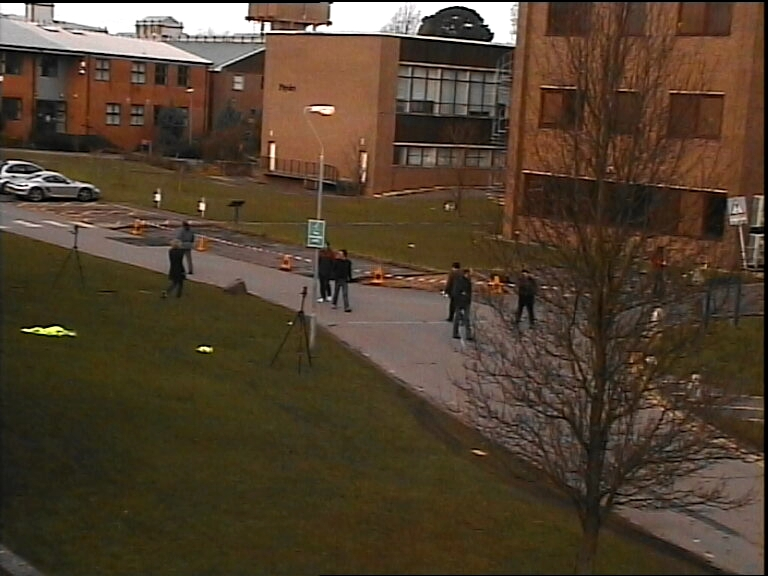
\includegraphics[height=2.85cm]{Figures/PETS2009-2}};
			\node at (8,0) [draw=black,ultra thick,inner sep=0pt]  {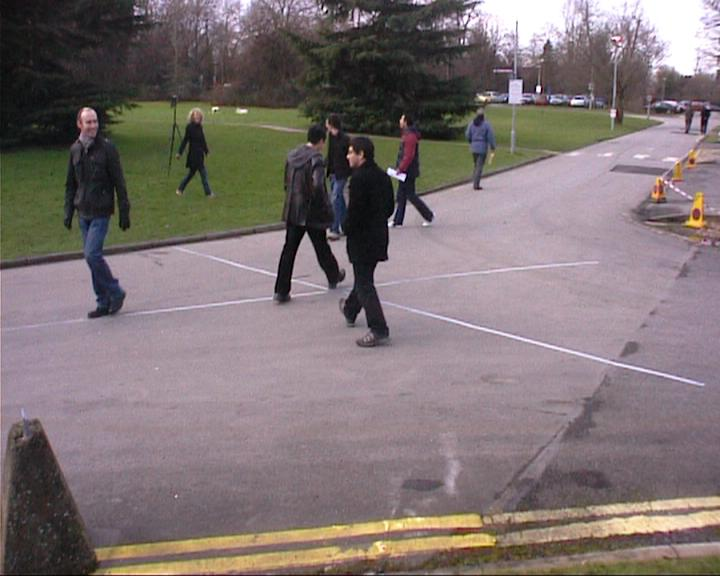
\includegraphics[height=2.85cm]{Figures/PETS2009-3}};
		\end{tikzpicture}
	\end{center}
\end{frame}

\begin{frame}
	\frametitle{Quantitative Evaluation on the People Domain}
	
	\begin{table}[!t]
		\renewcommand{\arraystretch}{1.3}
		\caption{Tracking performance on the PETS 2009 data set. MOTA (larger the better)
				 considers the number of missed detections, the number of false positives
				 and the switches of identities. MOTP (larger the better) considers the
				 precision of the detections.}
		\centering
		\vspace{0.2cm}
		
		\begin{tabular}{ccccc}
			\hline
			\hline
			\textbf{Method} & \textbf{MOTA} & \textbf{MOTP} & \textbf{Type} & \textbf{Real-Time} \\
			\hline
			Leal-Taix\'{e} \emph{et al.} \cite{Leal11} & 0.67 & 0.594 & Offline & NO \\
			\hline
			Berclaz \emph{et al.} \cite{Berclaz11} & 0.732 & 0.651 & Offline & NO \\
			\hline
			Sharma \emph{et al.} \cite{Sharma09} & 0.675 & 0.582 & Offline & NO \\
			\hline
			Breitenstein \emph{et al.} \cite{Berclaz11} & 0.745 & 0.563 & Online & NO \\
			\hline
			Yang \emph{et al.} \cite{Yang09} & 0.759 & 0.538 & Online & NO \\
			\hline
			PTracking & \textbf{0.814} & \textbf{0.652} & Online & \textbf{YES} \\
			\hline
		\hline
		\end{tabular}
	\end{table}
\end{frame}

\begin{frame}
	\frametitle{Application Field}
	
	\vspace{-0.12cm}
	
	\begin{itemize}
		\item Multi-Agent, Multi-Object
	\end{itemize}
	
	\vspace{-0.45cm}
	
	\begin{columns}[t]
		\only<1->
		{
			\column{0.75\textwidth}
			
			\begin{block}{Kinect}
				robots autonomously moving in an environment
			\end{block}
			
			\column{0.2\textwidth}
		}
	\end{columns}
	
	\centering
	\vspace{0.3cm}
	
	\begin{center}
		\begin{tikzpicture}
			\node at (0,0) [draw=black,ultra thick,inner sep=0pt]  {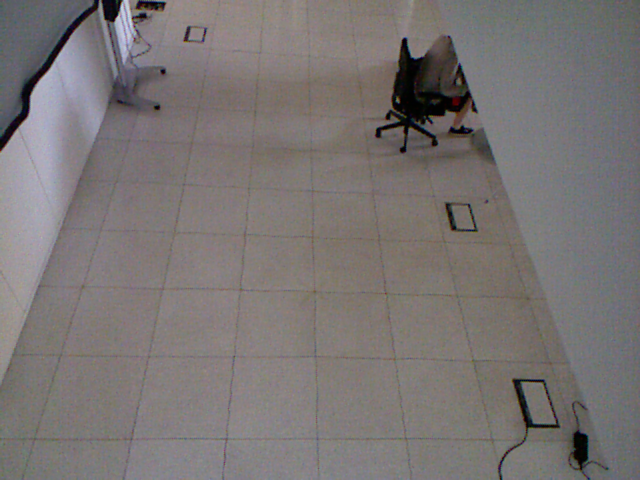
\includegraphics[height=2.9cm]{Figures/Kinect-1}};
			\node at (4,0) [draw=black,ultra thick,inner sep=0pt]  {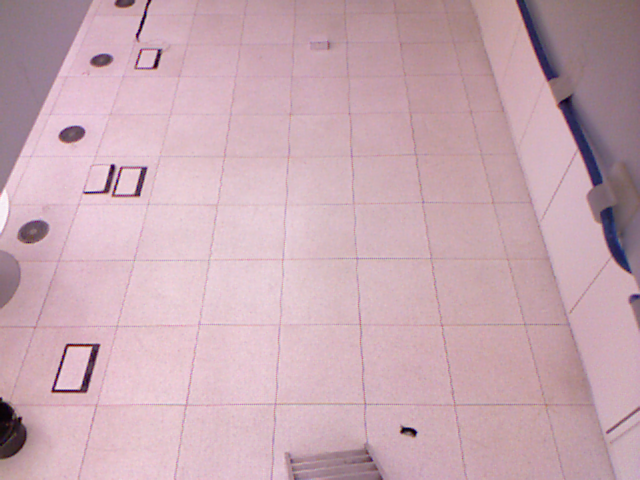
\includegraphics[height=2.9cm]{Figures/Kinect-2}};
			\node at (8,0) [draw=black,ultra thick,inner sep=0pt]  {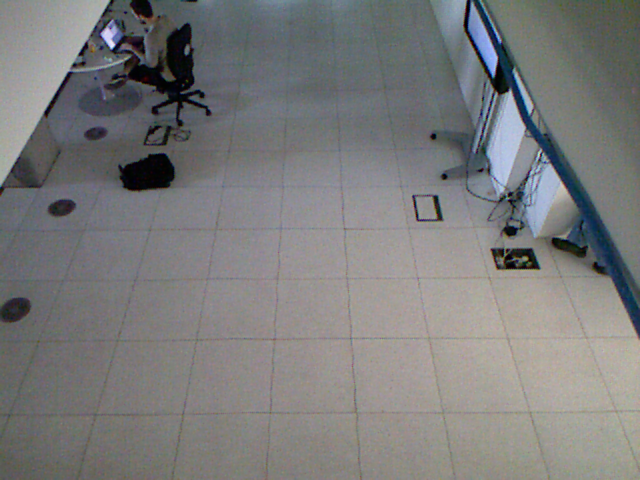
\includegraphics[height=2.9cm]{Figures/Kinect-3}};
		\end{tikzpicture}
	\end{center}
\end{frame}
